\documentclass{article}
\usepackage{amsmath, amssymb, amsthm}
% amsmath: equation*, amssymb: mathbb, amsthm: proof
\usepackage{moreenum}
\usepackage{mathtools}
\usepackage{url}
\usepackage{enumitem}
\usepackage{graphicx}
\usepackage{adjustbox}
\usepackage{subcaption}
\usepackage{booktabs} % toprule
\usepackage[mathcal]{eucal}
%% Definitions for Inference and Information
%% UPDATE: September 26, 2017 by Xiangxiang 
\newcommand{\theterm}{Fall 2017}
\usepackage{xeCJK}
\usepackage{bm}
\setCJKmainfont[AutoFakeBold]{SimSun}

\newcommand{\thecoursename}{
Tsinghua University\\
%\vspace*{0.1in}
现代信号处理
}
\newcommand{\studentID}{2017310711}
\newcommand{\courseheader}{
\vspace*{-1in}
\begin{center}
\thecoursename \\
\theterm
\vspace*{0.1in}
\hrule
\end{center}
}
\newcommand{\NP}{$\mathcal{NP}$}
\newcommand{\rvx}{\mathsf{x}}    % x, r.v.
\newcommand{\rvy}{\mathsf{y}}    % y, r.v.
\newcommand{\rvz}{\mathsf{z}}    % z, r.v.
\newcommand{\urvx}{\underline{\mathsf{x}}}    % x, r.v. vec
\newcommand{\urvy}{\underline{\mathsf{y}}}    % y, r.v. vec
\newcommand{\urvz}{\underline{\mathsf{z}}}    % z, r.v. vec
\newcommand{\defas}{\triangleq} %\coloneqq
\newcommand{\reals}{\mathbb{R}}
%\newcommand{\T}{\mathrm{T}}    % transpose

% \newcommand{\E}[1]{\mathbb{E}\left[{#1}\right]}
% \newcommand{\Prob}[1]{\mathbb{P}\left({#1}\right)}
\DeclareMathOperator*{\argmax}{arg\,max}
\DeclareMathOperator*{\argmin}{arg\,min}
\DeclareMathOperator*{\argsup}{arg\,sup}
\DeclareMathOperator*{\arginf}{arg\,inf}
\DeclareMathOperator{\Var}{Var}
\DeclareMathOperator{\Cov}{Cov}
\DeclareMathOperator{\MSE}{MSE}
\DeclareMathOperator{\In}{\mathbb{I}}
\DeclareMathOperator{\E}{\mathbb{E}}
\DeclareMathOperator{\Prob}{\mathbb{P}}
\DeclareMathOperator{\sign}{sign}
\DeclareMathOperator\err{err}
\DeclareMathOperator\conv{conv}
\newcommand\independent{\protect\mathpalette{\protect\independenT}{\perp}}
\def\independenT#1#2{\mathrel{\rlap{$#1#2$}\mkern2mu{#1#2}}}
\usepackage{listings}
\usepackage{xcolor}
\definecolor{dkgreen}{rgb}{0,0.6,0}
\definecolor{gray}{rgb}{0.5,0.5,0.5}
\definecolor{mauve}{rgb}{0.58,0,0.82}

\lstset{
  frame=tb,
  aboveskip=3mm,
  belowskip=3mm,
  showstringspaces=false,
  columns=flexible,
  framerule=1pt,
  rulecolor=\color{gray!35},
  backgroundcolor=\color{gray!5},
  basicstyle={\small\ttfamily},
  numbers=none,
  numberstyle=\tiny\color{gray},
  keywordstyle=\color{blue},
  commentstyle=\color{dkgreen},
  stringstyle=\color{mauve},
  breaklines=true,
  breakatwhitespace=true,
  tabsize=3,
  title=\lstname
}




\begin{document}
\courseheader
\begin{center}
  \underline{LMS和RLS仿真实验报告} \\
\end{center}
\begin{flushleft}
  赵丰\quad \studentID\hfill
  \today
\end{flushleft}
\hrule

\vspace{2em}

\flushleft
\rule{\textwidth}{1pt}
\begin{itemize}
\item {\bf Acknowledgments: \/} 
  This coursework refers to textbook.  
\item {\bf Collaborators: \/}
  \begin{itemize}
  \item (1) was solved with the help from my roommate 周豪宇
  \end{itemize}
\end{itemize}
\rule{\textwidth}{1pt}

\vspace{2em}

%\title{EM算法上机作业}
%\author{赵丰,2017310711}
%\maketitle
\begin{enumerate}[label={(\arabic*)}]
\item LMS算法实现自适应均衡器,matlab代码如下所示
\lstinputlisting[language=matlab]{lms_system.m}
针对三组不同的白噪声方差值$\sigma^2$,取LMS的迭代步长$\mu=0.05$,作出一次实验误差平方随数字时间的变化如下图所示:

\begin{figure}[!ht]
\centering
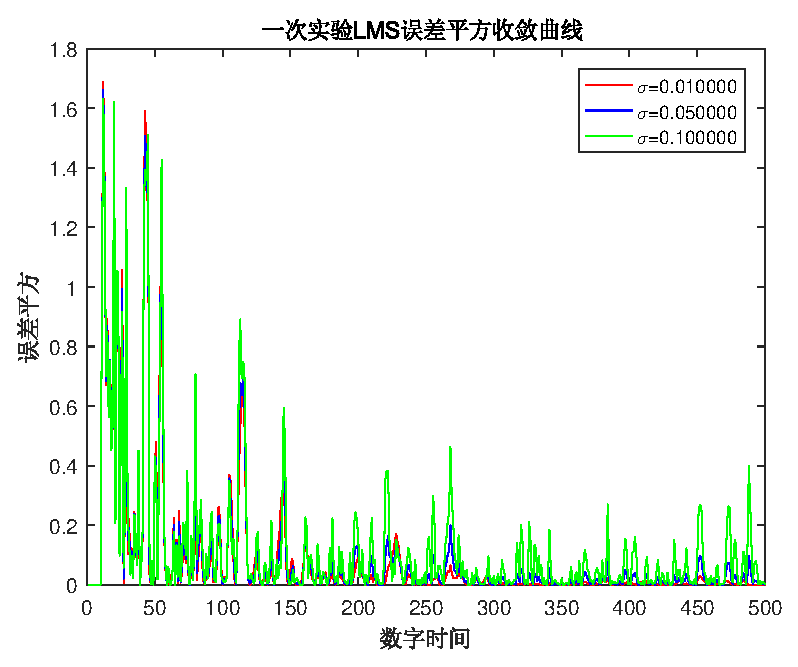
\includegraphics[width=10cm]{lml_one_time.eps}
\caption{}\label{fig:1}
\end{figure}

由图\ref{fig:1}可以看到,对于给定的迭代步长,噪声越大,单次实验误差的平方相对抖动,但噪声在一定范围内误差平方有减小的趋势。

针对给定的白噪声方差值$\sigma^2=0.05^2$,取三组不同的LMS的迭代步长$\mu$,作出20次实验误差平方的平均值(可作为$E(e(n))$的估计)
随数字时间的变化如下图所示:

\begin{figure}[!ht]
\centering
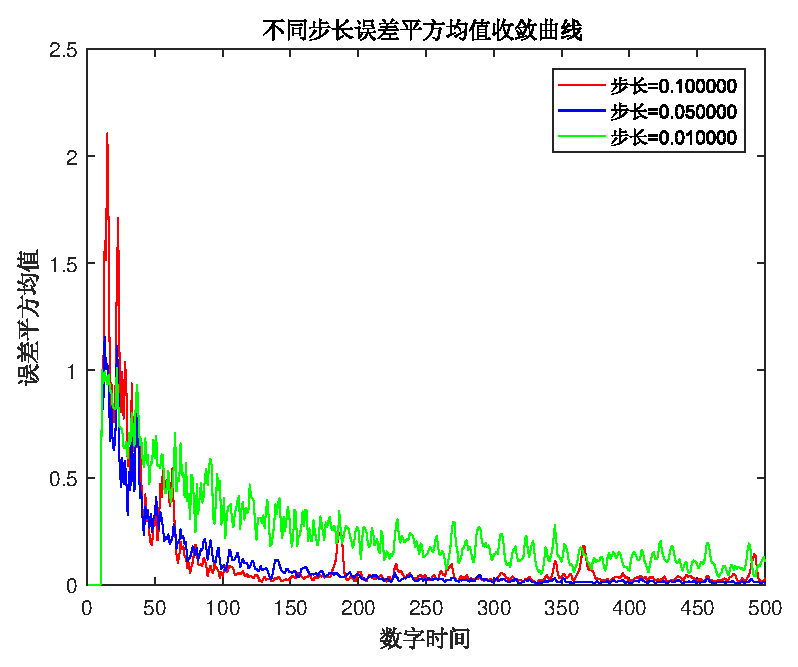
\includegraphics[width=10cm]{lml_many_times.eps}
\caption{}\label{fig:2}
\end{figure}

由图\ref{fig:1}可以看到,对于给定的白噪声方差值,$\mu$越小收敛速度越慢,但收敛的稳定性越好。
$\mu$较大时收敛速度虽快,但由于$e(n)$方差较大,20次平均不足以反映$E(e(n))$,所以抖动较为明显。

对于步长为0.05的情形,自适应均衡器的各阶系数如下表如示:
\begin{table}[!ht]
\centering
\caption{自适应均衡器滤波器系数}
\begin{adjustbox}{max width=\textwidth}
\begin{tabular}{|c|c|c|c|c|c|c|c|c|c|c|c|}
\hline
序号 & 1 & 2 & 3 & 4 & 5 & 6 & 7 & 8 & 9 & 10 & 11\\
\hline
20次平均 &
0.0151 &-0.0653 &0.1915 &-0.5378 &1.4567 &-0.5377 &0.1912 &-0.0645 &0.0173 &-0.0054 &0.0025
\\
\hline
\end{tabular}
\end{adjustbox}
\end{table}
将上表的序列与$[0.3,0.9,0.3]$作卷积,得到长为13的序列,只有倒数第8位接近1,其余位接近0。这说明在信噪比较大的情况下
采用11阶LMS滤波可以较好的恢复原信号。

本题如采用Wiener滤波,由于11阶的FIR可以形成对3阶FIR逆系统的好的近似,
所以$J_{\min}$接近0,对于实际情形,由于500组观测数据(较多),可以通过统计的方法形成对自相关和互相关的好的近似,因此
使用LMS算法也能使$e(n)$误差接近0。


\item RLS算法实现自适应均衡器,matlab代码如下所示
\lstinputlisting[language=matlab]{rls_system.m}
针对$\mu=0.01,\sigma=0.05$的情况,分别作出LMS和RLS算法20次实验误差平方的平均值随数字时间的变化如下图所示:

\begin{figure}[!ht]
\centering
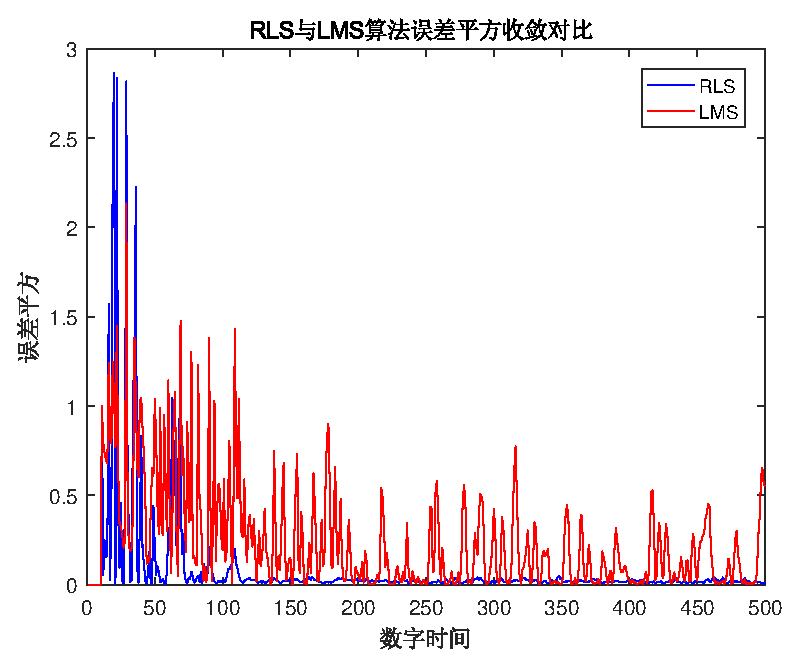
\includegraphics[width=10cm]{compare.eps}
\caption{}\label{fig:3}
\end{figure}

由图\ref{fig:3}可以看到,RLS算法收敛速度远快于LMS算法。

本次仿真使用的均衡器系统的初始化代码和绘图代码如下:
\lstinputlisting[language=matlab]{launcher.m}

\end{enumerate}
\end{document}

